\scanpage{43}

\noindent
\begin{tabular}{@{}c@{\qquad\qquad}l@{}}
$\mathcal H^1(X;A)$ & $\operatorname{Ext}^1(A,\operatorname{Pic})$\\[-1mm]
\begin{tikzpicture}[x=1cm,y=1cm]
\draw (0,.55) .. controls (-.03,.34) and (.03,.12) .. (.07,0);
\end{tikzpicture} &\\[-1mm]
\unsure{pt singuliers|pt singulier} &
\end{tabular}

\[
\begingroup
\setbox0=\hbox{$\displaystyle\mathcal H^1(X,G)\simeq\operatorname{Hom}(D(G),\operatorname{\underline{Pi}c}_X)$}
\hbox{\rlap{\begin{tikzpicture}[overlay,baseline=0pt]
\draw (-8pt,24pt) -- (\dimexpr\wd0-16pt\relax,22pt) -- (\dimexpr\wd0-19pt\relax,20pt);
\draw (-6pt,17pt) -- (-5pt,-12pt) -- (\dimexpr\wd0+8pt\relax,-11pt) -- (\dimexpr\wd0+9pt\relax,-8pt);
\draw (\dimexpr\wd0+12pt\relax,16pt) -- (\dimexpr\wd0+10pt\relax,-5pt) -- (\dimexpr\wd0+7pt\relax,-6pt);
\end{tikzpicture}}\box0}
\endgroup
\]

\figure{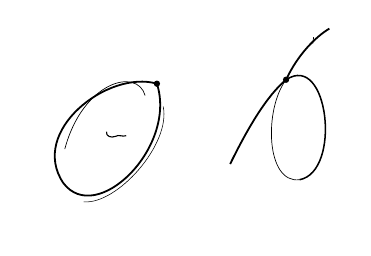
\begin{tikzpicture}[x=1cm,y=1cm]
\draw[line width=.65pt] (1.14,1.40) .. controls (.52,1.58) and (-.49,.80) .. (-.05,.14)
.. controls (.37,-.42) and (1.40,.59) .. (1.14,1.40);
\draw[line width=.25pt] (-.03,.57) .. controls (.20,1.43) and (.89,1.61) .. (.99,1.25);
\fill (1.14,1.40) circle (.04);
\draw (.50,.79) .. controls (.49,.73) and (.56,.71) .. (.61,.73) .. controls (.66,.76) and (.70,.72) .. (.75,.74);
\draw[line width=.2pt] (1.22,1.11) .. controls (1.32,.63) and (.63,-.14) .. (.21,-.10);
\draw[line width=.65pt] (2.07,.38) .. controls (2.30,.85) and (2.54,1.25) .. (2.78,1.45);
\draw[line width=.55pt] (2.78,1.45) .. controls (3.32,1.81) and (3.49,.28) .. (2.95,.18);
\draw[line width=.25pt] (2.95,.18) .. controls (2.52,.13) and (2.50,1.08) .. (2.78,1.45);
\draw[line width=.65pt] (2.78,1.45) .. controls (2.93,1.77) and (3.15,1.99) .. (3.33,2.10);
\draw[line width=.25pt] (3.13,1.99) -- (3.12,1.91);
\fill (2.78,1.45) circle (.04);
\end{tikzpicture}}

\[
\mathcal H^i(X,D(G))\simeq\operatorname{Ext}^i(G,\underline{\operatorname{Pic}}_X)
\]

\[
\operatorname{Ext}^i_X(f^!(G),G_m,)\simeq
\operatorname{Ext}^i_Y(G,f_{\unsure{!|\cdot}}(G_m))
\]

\reversemarginpar
\margin{\begin{tikzcd}[ampersand replacement=\&,column sep=small,row sep=0pt]
\&X\\
f\&\unsure{\vert|\downarrow}\\
\&Y
\end{tikzcd}}
\normalmarginpar
\[
\begingroup
\setbox0=\hbox{$\displaystyle
\underline{\operatorname{Ext}}^i_X(f^*(G_{\bullet}),H^{\bullet})\simeq
\underline{\operatorname{Ext}}^i_Y(G_{\bullet},f_!(H^{\bullet}))$}
\hbox{\rlap{\begin{tikzpicture}[overlay,baseline=0pt]
\draw (-8pt,25pt) -- (\dimexpr\wd0+7pt\relax,24pt);
\draw (-7pt,21pt) -- (-6pt,-13pt) -- (\dimexpr\wd0+7pt\relax,-12pt);
\draw (-6pt,-13pt) -- (-3pt,-10pt);
\draw (\dimexpr\wd0+12pt\relax,17pt) -- (\dimexpr\wd0+11pt\relax,-8pt) -- (\dimexpr\wd0+8pt\relax,-7.5pt);
\end{tikzpicture}}\box0}
\endgroup
\]

\[H=G_m\]

\[
\underline{\operatorname{Ext}}^i_X
\bigl(\underset{\substack{\uparrow\\[-.4ex]\inserted{R}}}{f^*}(G),G_m\bigr)
\simeq\underline{\operatorname{Ext}}^i_Y\bigl(G,
\overset{\text{les \unsure{supérieurs}}}{
\begingroup
\setbox0=\hbox{$\displaystyle\underline{\operatorname{Pic}}^{\bullet}_{X/Y}$}
\hbox{\rlap{\begin{tikzpicture}[overlay,baseline=0pt]
\draw (-5pt,9pt) .. controls (0pt,22pt) and (\dimexpr\wd0+12pt\relax,22pt) .. (\dimexpr\wd0+11pt\relax,3pt)
.. controls (\dimexpr\wd0+12pt\relax,-19pt) and (-10pt,-21pt) .. (-6pt,-2pt);
\draw (20pt,-8pt) -- (20pt,-27pt);
\draw (23pt,-11pt) -- (23pt,-30pt);
\end{tikzpicture}}\box0\kern10pt}
\endgroup}
\bigr)
\]

\noindent\hspace*{.27\linewidth}
$\deleted{H^{\unsure{i}}(X,}$
\hspace{1.2cm}
\raisebox{1.5ex}[0pt][0pt]{\begin{tikzpicture}[overlay,baseline=0pt]
\draw (0pt,9pt) .. controls (0pt,-8pt) and (1pt,-19pt) .. (6pt,-27pt);
\draw (4pt,10pt) .. controls (3pt,-9pt) and (4pt,-27pt) .. (5pt,-31pt) -- (2pt,-31pt);
\end{tikzpicture}}
\par\medskip

\[
\begingroup
\setbox0=\hbox{$\displaystyle G\ \text{\uline{\unsure{affine|fini}}},\ \text{alors}\quad
H^i(X,D(G))\Longleftarrow
\deleted{\unsure{\mathcal H|E}}\operatorname{Ext}^{\unsure{p|1|i}}(G,\operatorname{Pic}^{\unsure{(q)|(1)}}_{X/Y})$}
\hbox{\rlap{\begin{tikzpicture}[overlay,baseline=0pt]
\draw (-9pt,24pt) -- (\dimexpr\wd0+12pt\relax,25pt);
\draw (-6pt,14pt) .. controls (-8pt,-5pt) and (-5pt,-13pt) .. (9pt,-13pt)
-- (\dimexpr\wd0+12pt\relax,-12pt);
\end{tikzpicture}}\box0}
\endgroup
\]

\[
\begin{array}{rll}
i=0&H^0(X,D(G))=&\deleted{\operatorname{Hom}}D(G)\\
i=1&H^1(X,D(G))=&\deleted{\unsure{\operatorname{Ex}}}\operatorname{Hom}(G,\operatorname{Pic}^{(1)})\\
i=2&H^2\unsure{(}X,D(G))\mathrel{\substack{\unsure{\#|\neq}\\\hphantom{\#}!}}&
\operatorname{Ext}^1(G,\operatorname{Pic}^{(1)}_{X/Y})+
\operatorname{Hom}(G,\operatorname{\underline{P}ic}^{\unsure{(2}}_X
\end{array}
\]

\figure{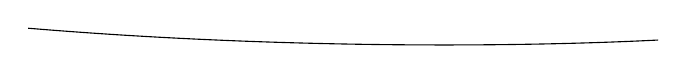
\begin{tikzpicture}[x=1cm,y=1cm]
\draw (0,.15) .. controls (3,-.1) and (6,-.1) .. (8,0);
\end{tikzpicture}}

\noindent $G$ \unsure{abélien}\unsure{,} \unsure{alors|dans} $\unsure{\mathcal A|\deleted{H}|H}$
\[
H^{i-1}(X,G')\Longleftarrow
\operatorname{Ext}^{p}_{\unsure{\mathcal A|q}}(G,\operatorname{Pic}^{\unsure{q|1|?}}_{X/Y})
\]

\[
\begin{array}{rl}
i\unsure{=}0&0=0\\
i=1&H^0(X,G')=
\end{array}
\]
\margin{42}
